\documentclass[a4paper,10pt]{article}

% рисунки
\usepackage{graphicx}

\usepackage[T2A]{fontenc}
\usepackage[utf8]{inputenc}
\usepackage[english,russian]{babel}
\usepackage{amssymb}

\RequirePackage{caption}
\DeclareCaptionLabelSeparator{defffis}{ — }
\captionsetup{justification=centering,labelsep=defffis}

\usepackage{caption} \captionsetup[table]{labelsep=endash,justification=justified,singlelinecheck=false,font=normalsize}

\usepackage{amsmath,amsfonts,amssymb,amsthm,mathtools}



\begin{document}
  
\begin{center}
  \section*{Лабораторная работа №3.6.1 \\Спектральный анализ электрических сигналов\\Джокер Бэтмен, Б02-000, 18.09.2021}
\end{center}  

\vspace{5mm}
\section*{Введение}

\begin{flushleft}
  \textbf{Цель работы:} изучить спектральный состав периодических электрических сигналов.

\end{flushleft}

\begin{flushleft}
  \textbf{В работе используются:} аналоговый анализатор спектра, генератор прямоугольных импульсов и сигналов специальной формы, осциллограф.

\end{flushleft}

\section*{Теоретическая справка}

Периодическая функция может быть представлена в виде бесконечного ряда гармонических функций -- ряда Фурье:\[f(t)=\sum_{n=-\infty}^{+\infty}c_ne^{in\omega_0t}\ \text{или}\ f(t)=\sum_{n=0}^{+\infty}a_n\cos{\left(n\omega_0t+\varphi_n\right)}.\]Здесь $\omega_0=\frac{2\pi}{T}$, где $T$ -- период функции $f(t)$. Коэффициенты $\left\{c_n\right\}$ могут быть найдены по формуле:\[c_n=\frac{1}{T}\int_0^Tf(t)e^{-in\omega_0t}\text{d}t.\]Наборы коэффициентов разложения в комплексной $\left\{c_n\right\}$ и действительной $\left\{a_n,\varphi_n\right\}$ формах связаны соотношением:\[a_n=2\left|c_n\right|,\ \varphi_n=\arg{c_n}.\]

В качестве простейшего спектрального анализатора можно использовать высокодобротный колебательный контур с подстраиваемой ёмкостью или индуктивностью. Такой контур усиливает те гармоники входного сигнала $f(t)$, частота которых близка к резонансной $\nu_0=\frac{1}{2\pi\sqrt{LC}}$ и практически не реагирует на частоты, далёкие от $\nu_0$. С точки зрения преобразования гармоник колебательный контур является узкополосным \textit{фильтром} с шириной полосы пропускания порядка $\Delta\nu\sim\frac{\nu_0}{Q}$, где $Q=\frac{1}{R}\sqrt{\frac{L}{C}}\gg1$ -- его добротность. Амплитуда колебаний в контуре пропорциональна амплитуде $\left|c\left(\nu_0\right)\right|$ гармоники в спектре функции $f(t)$, частота которой совпадает с $\nu_0$. Таким образом, меняя резонансную частоту контура, можно "просканировать" весь спектр входного сигнала.

\section*{Экспериментальная установка}

\subsection*{Исследование спектра периодической последовательности прямоугольных импульсов}

Экспериментальная установка для исследования спектра периодической последовательности прямоугольных импульсов представлена на рисунке \Ref{Device}. Сигнал с выхода генератора прямоугольных импульсов Г5-54 подаётся на вход анализатора спектра и одновременно -- на вход Y осциллографа. С генератора импульсов на осциллограф подаётся также сигнал синхронизации, запускающий ждущую развёртку осциллографа. При этом на экране осциллографа можно наблюдать саму последовательность прямоугольных импульсов, а на экране ЭЛТ анализатора спектра -- распределение амплитуд спектральных составляющих этой последовательности.

\begin{figure}[h]
	\centering
	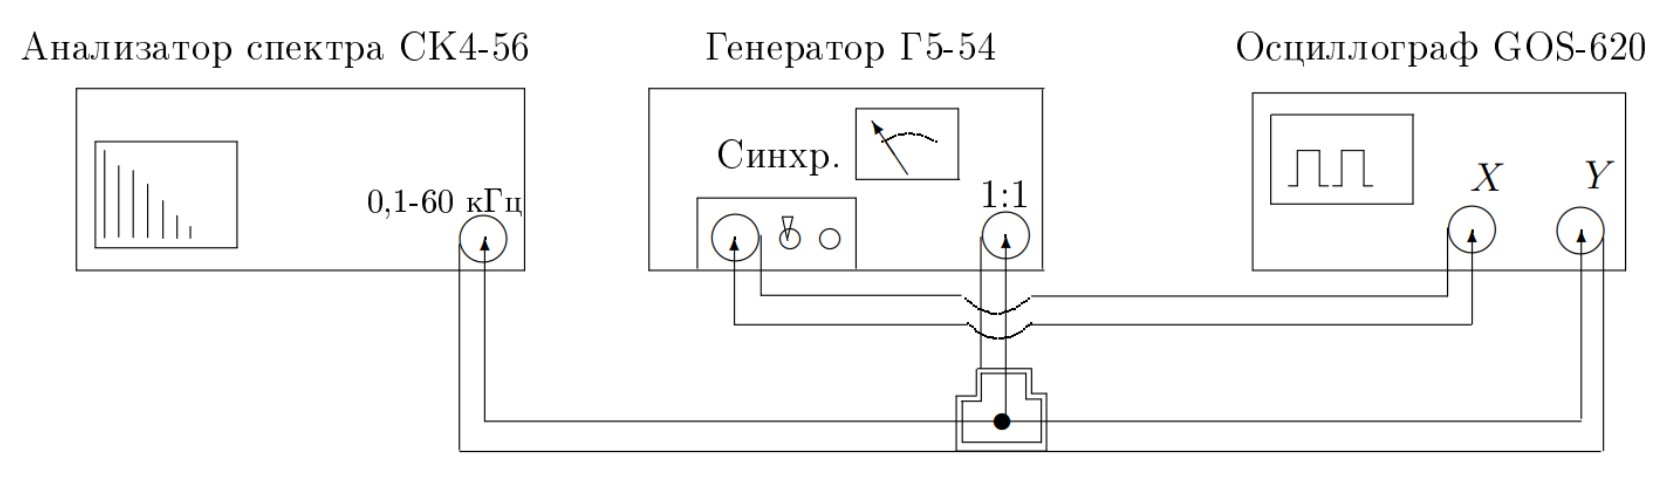
\includegraphics[scale=0.27]{Device}
	\caption{Схема для исследования спектра периодической последовательности прямоугольных импульсов} \label{Device}
\end{figure}

В наблюдаемом спектре отсутствует информация об амплитуде нулевой гармоники, т.е. о величине постоянной составляющей; её местоположение (начало отсчёта шкалы частот) отмечено небольшим вертикальным выбросом.

\subsection*{Исследование спектра периодической последовательности цугов гармонических колебаний}

\begin{figure}[h]
	\centering
	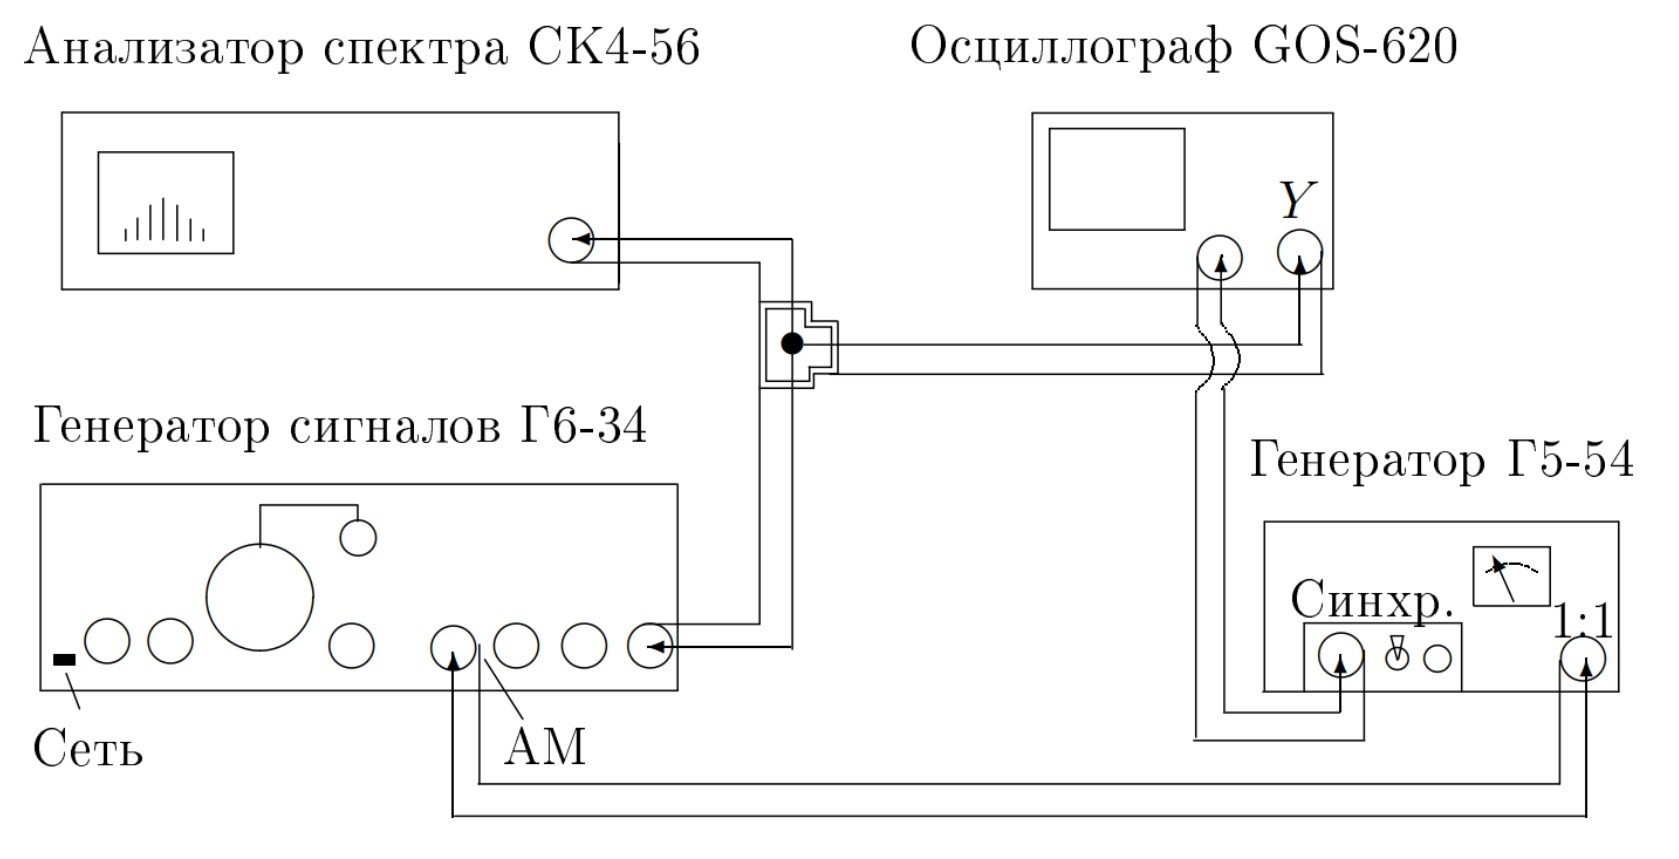
\includegraphics[scale=0.27]{Device_2}
	\caption{Схема для исследования спектра периодической последовательности цугов высокочастотных колебаний} \label{Device_2}
\end{figure}

Исследование спектра периодически чередующихся цугов гармонических колебаний проводится по схеме, изображённой на рисунке \Ref{Device_2}. Генератор Г6-34 вырабатывает синусоидальные колебания высокой частоты. На вход АМ (амплитудная модуляция) генератора Г6-34 подаются прямоугольные импульсы с генератора Г5-54 и синусоида модулируется -- "нарезается" на отдельные куски -- \textit{цуги}. Эти цуги с выхода генератора Г6-34 поступают на вход спектроанализатора и одновременно на вход Y осциллографа. Сигнал синхронизации подаётся на осциллограф с генератора импульсов.

\subsection*{Исследование спектра гармонических сигналов, модулированных по амлитуде}

Схема для исследования амплитудномодулированного сигнала представлена на рисунке \Ref{Device_3}. В генератор сигналов генератора встроен модуляционный генератор, который расположен в левой части Г6-34. Синусоидальный сигнал с частотой модуляции $f_{\text{мод}}=1~\text{кГц}$ подаётся с модуляционного генератора на вход АМ (амплитудная модуляция) генератора, вырабатывающего синусоидальный сигнал высокой частоты (частота несущей $\nu_0=25~\text{кГц}$). Амплитудно-модулированный сигнал с основного выхода генератора поступает на осциллограф и на анализатор спектра.

\begin{figure}[h]
	\centering
	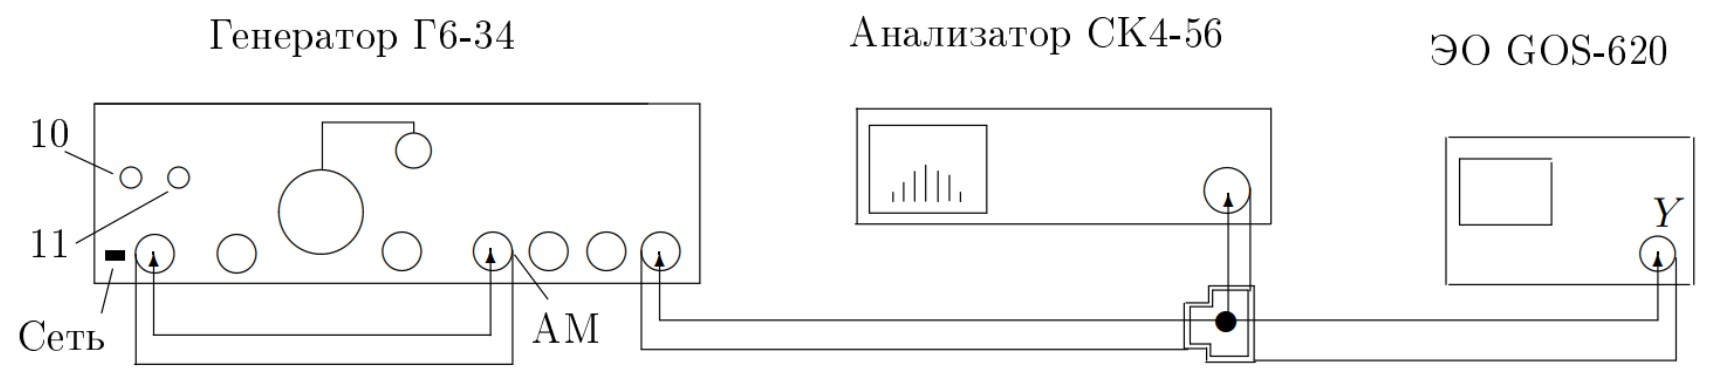
\includegraphics[scale=0.27]{Device_3}
	\caption{Схема для исследования спектра высокочастотного гармонического сигнала, промодулированного по амплитуде низкочастотным гармоническим сигналом} \label{Device_3}
\end{figure}

\section*{Ход работы}

\subsection*{А. Исследование спектра периодической последовательности прямоугольных импульсов}

Соберём схему согласно \Ref{Device}, включим в сеть генератор Г5-54 и подготовим установку к измерениям. Установим на анализаторе спектра режим работы с однократной развёрткой и получим на экране спектр импульсов с параметрами $f_{повт}=10^3~\text{Гц}$; $\tau=25~\text{мкс}$; $m_x=5~\frac{\text{кГц}}{\text{дел}}$. Увеличим $\tau$ вдвое при неизменном $f_{повт}=1~\text{кГц}$ и посмотрим, как меняется при этом спектр (величины $\Delta\nu$ и $\delta\nu$). Видим, что $\Delta\nu$ уменьшается вдвое при неизменной $\delta\nu$. Теперь увеличим вдвое $f_{повт}$ при неизменном $\tau$. Видим, что $\Delta\nu$ при этом не изменится (огибающая останется прежней), однако в два раза увеличится $\delta\nu$.

Проведём измерения зависимости ширины спектра от длительности импульса $\Delta\nu\left(\tau\right)$ при увеличении $\tau$ от 25 до 200 мкс при $f_{повт}=1~\text{кГц}$ и $m_x=5~\frac{\text{кГц}}{\text{дел}}$. Занесём результаты измерений в таблицу \Ref{Table_A}. Проведём также оценку погрешностей. Так как данные получены при постоянной $f_{повт}$, то и $\delta\nu$ для них постоянна. Отсюда следует, что абсолютную погрешность определения $\Delta\nu$ можно принять равной отношению расстояния между соседними линиями спектра к ширине всей шкалы спектрометра, т.е. $\varepsilon_{\Delta\nu}=\frac{1~\text{кГц}}{50~\text{кГц}}=2,0~\%$. Погрешность $\Delta\tau$ равна половине цены деления шкалы, по которой выставляется $\tau$, для $\tau=25~\text{мкс}$ она равна $\Delta\tau=0,5~\text{мкс}$, для $\tau=50\ldots75~\text{мкс}$ -- $\Delta\tau=2,5~\text{мкс}$, а для $\tau=100\ldots200~\text{мкс}$ -- $\Delta\tau=5,0~\text{мкс}$. Отсюда несложно посчитать и погрешности $\sigma_{\frac{1}{\tau}}$. Занесём все эти погрешности в таблицу \Ref{Table_A}.

\begin{table}[h]
	\centering
	\caption{Зависимость ширины спектра $\Delta\nu$ от длительности импульса $\tau$} \label{Table_A}
	\begin{tabular}{|c|c|c|c|c|c|c|c|c|}
		\hline
		$\tau$, мкс & 25,0 & 50,0 & 75,0 & 100,0 & 125,0 & 150,0 & 175,0 & 200,0 \\ \hline
		$\frac{1}{\tau}$, кГц & 40,0 & 20,0 & 13,3 & 10,0 & 8,0 & 6,7 & 5,7 & 5,0 \\ \hline
		$\sigma_{\frac{1}{\tau}}$, кГц & 0,8 & 1,0 & 0,4 & 0,5 & 0,3 & 0,2 & 0,2 & 0,1 \\ \hline
		$\Delta\nu$, кГц & 40,0 & 20,0 & 13,5 & 10,0 & 8,0 & 6,5 & 5,7 & 5,0 \\ \hline
		$\sigma_{\Delta\nu}$, кГц & 1,0 & 0,5 & 0,3 & 0,3 & 0,2 & 0,2 & 0,1 & 0,1 \\ \hline
	\end{tabular}
\end{table}

Приступим теперь к обработке полученных данных. Построим график $\Delta\nu\left(\frac{1}{\tau}\right)$. Видим, что точки очень хорошо ложатся на прямую, поэтому найти наклон графика и его погрешность можно, используя МНК, и затем, используя этот результат, провести на графике прямую. Получим $k=1,001\pm0,016$, откуда с хорошей точностью можем заключить, что $\tau\Delta\nu=1$, что экспериментально доказывает соотношение неопределённостей. График приведён ниже на рисунке \Ref{Plot_A}.

\begin{figure}[h]
	\centering
	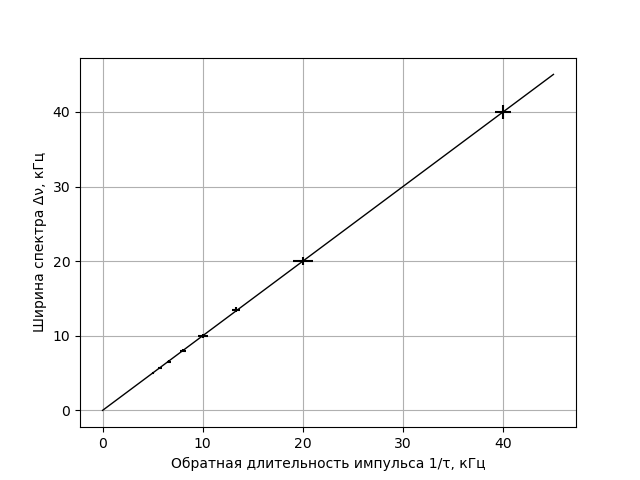
\includegraphics[scale=0.75]{Plot_A}
	\caption{График зависимости ширины спектра $\Delta\nu$ от обратной длительности импульса $\frac{1}{\tau}$. Прямая проведена с помощью МНК} \label{Plot_A}
\end{figure}

Сделаем также ровные и чёткие фотографии спектров с параметрами $f_{повт}=1~\text{кГц}$, $m_x=5~\frac{\text{кГц}}{\text{дел}}$ и (1) $\tau=50~\text{мкс}$, (2) $\tau=100~\text{мкс}$. Для улучшения контраста и размера значимой части изображения обрежем фотографии и инвертируем на них цвета. Полученные результаты (рисунки \Ref{Spectr_1} и \Ref{Spectr_2}) приведены ниже.

\begin{figure}[h]
	\centering
	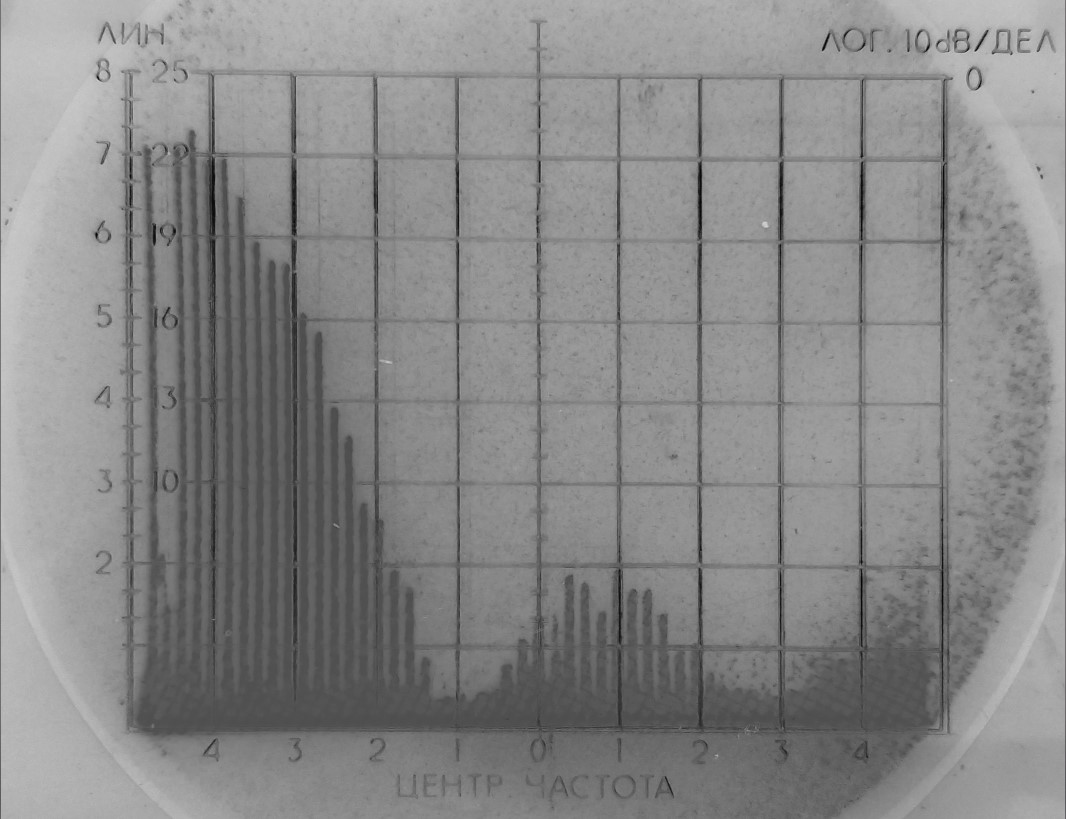
\includegraphics[scale=0.40]{Spectr_1}
	\caption{Фотография спектра с параметрами $f_{повт}=1~\text{кГц}$, $m_x=5~\frac{\text{кГц}}{\text{дел}}$, $\tau=50~\text{мкс}$} \label{Spectr_1}
	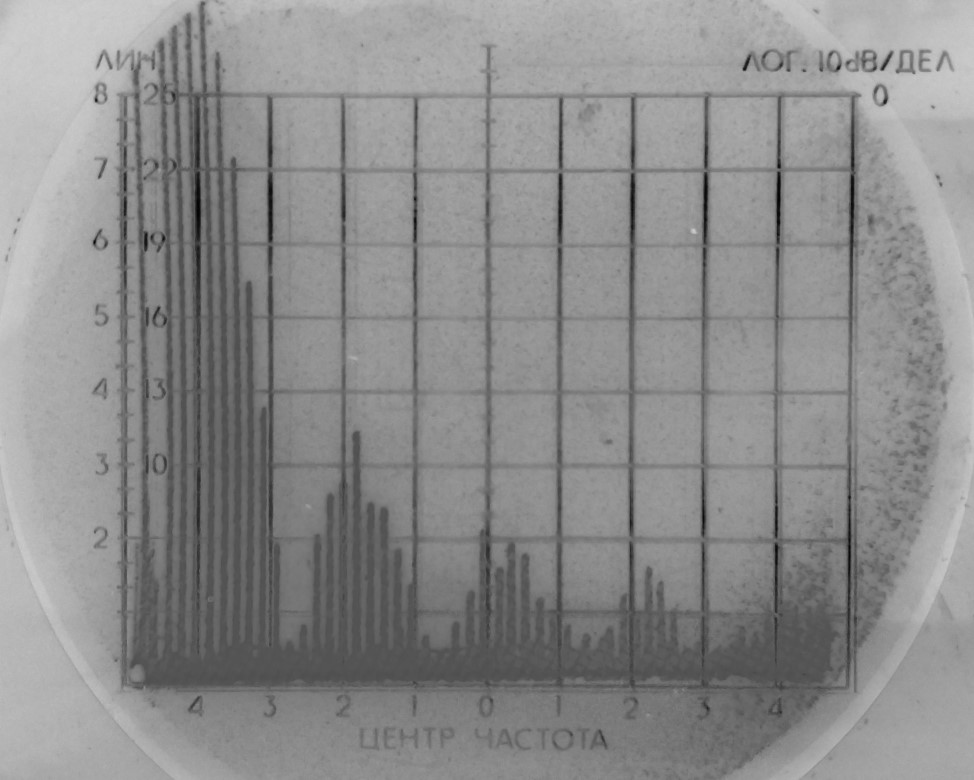
\includegraphics[scale=0.44]{Spectr_2}
	\caption{Фотография спектра с параметрами $f_{повт}=1~\text{кГц}$, $m_x=5~\frac{\text{кГц}}{\text{дел}}$, $\tau=100~\text{мкс}$} \label{Spectr_2}
\end{figure}

\subsection*{Б. Исследование спектра периодической последовательности цугов гармонических колебаний}

Соберём теперь схему, изображённую на рисунке \Ref{Device_2} и подготовим установку к работе. Установим частоту несущей $\nu_0=25~\text{кГц}$. Сначала проведём наблюдения изменения спектра при увеличении $\tau$ вдвое (с $\tau=50~\text{мкс}$ до $\tau=100~\text{мкс}$) при неизменных $f_{повт}=1~\text{кГц}$ и $m_x=5~\frac{\text{кГц}}{\text{дел}}$. Видим, что спектр остаётся симметричным относительно одной и той же точки, однако "сжимается" к ней вдвое. Теперь пронаблюдаем за изменением спектра при изменении несущей частоты $\nu_0$ (при значениях $\nu_0=25~\text{кГц}$, $\nu_0=10~\text{кГц}$ и $\nu_0=40~\text{кГц}$) при постоянных $\tau=100~\text{мкс}$, $f_{повт}=1~\text{кГц}$ и $m_x=5~\frac{\text{кГц}}{\text{дел}}$. Видим, что в этом случае спектр не меняет свою форму, однако его центр смещается в соответсвии с изменением частоты несущей.

При фиксированной длительности импульсов $\tau=50~\text{мкс}$ исследуем зависимость расстояния $\delta\nu$ между соседними спектральными компонентами от частоты повторения $f_{\text{повт}}$. Измерения будем проводить в диапазоне $f_{повт}=1\ldots8~\text{кГц}$ при масштабе $m_x=5~\frac{\text{кГц}}{\text{дел}}$, являющимся наиболее удобным для измерений. Полученные результаты занесём в таблицу \Ref{Table_B}. Проведём также оценку погрешностей. Абсолютную погрешность $\delta\nu$  можно оценть как отношение половины цены деления сетки шкалы спектрометра к её ширине, тогда $\varepsilon_{\delta\nu}=\frac{2,5~\text{кГц}}{50~\text{кГц}}=5,0~\%$. Погрешность определения $f_{повт}$ равна половине цены деления шкалы, по которой она выставляется, и для $f_{повт}=1\ldots3~\text{кГц}$ она равна $\Delta f_{повт}=0,02~\text{кГц}$, а для $f_{повт}=4\ldots8~\text{кГц}$ -- $\Delta f_{повт}=0,1~\text{кГц}$. Занесём все эти погрешности в таблицу \Ref{Table_B}.

\begin{table}[h]
	\centering
	\caption{Зависимость ширины спектра $\Delta\nu$ от длительности импульса $\tau$} \label{Table_B}
	\begin{tabular}{|c|c|c|c|c|c|c|}
		\hline
		$f_{повт}$, кГц & 1,00 & 2,0 & 3,0 & 4,0 & 6,0 & 8,0 \\ \hline
		$\sigma_{f_{повт}}$, кГц & 0,02 & 0,1 & 0,1 & 0,1 & 0,1 & 0,1 \\ \hline
		$\delta\nu$, кГц & 1,00 & 2,00 & 3,00 & 4,0 & 6,0 & 8,0 \\ \hline
		$\sigma_{\delta\nu}$, кГц & 0,05 & 0,1 & 0,2 & 0,2 & 0,3 & 0,4 \\ \hline
	\end{tabular}
\end{table}

Приступим теперь к обработке полученных данных. Построим график $\delta\nu\left(f_{\text{повт}}\right)$. Видим, что точки очень хорошо ложатся на прямую, поэтому найти наклон графика и его погрешность можно, используя МНК, и затем, используя этот результат, провести на графике прямую. Получим $k=1,00\pm0,04$. График приведён ниже на рисунке \Ref{Plot_B}. Таким образом, с хорошей точностью можем сказать, что $\delta\nu=f_{повт}$, что совпадает с теоретическим предсказанием. Можно сделать вывод, что \textit{при стремлении частоты повторнения к нулю спектр переходит из дискретного в непрерывный}.

\begin{figure}[h]
	\centering
	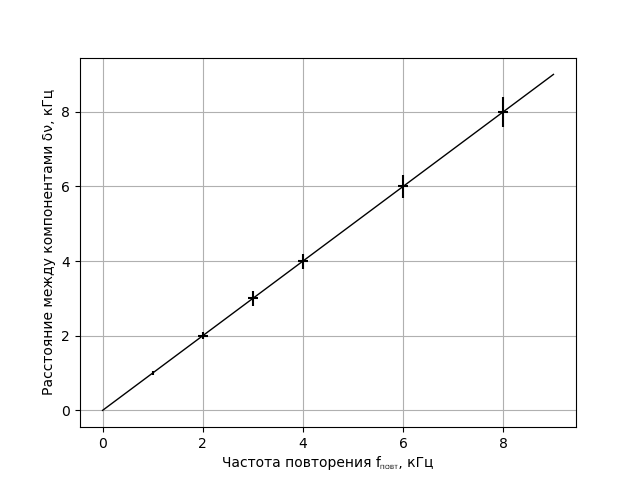
\includegraphics[scale=0.75]{Plot_B}
	\caption{График зависимости расстояния $\delta\nu$ между соседними спектральными компонентами от частоты повторения $f_{повт}$. Прямая проведена с помощью МНК} \label{Plot_B}
\end{figure}

Сделаем фотографии спектров с параметрами $\tau=100~\text{мкс}$, $m_x=5~\frac{\text{кГц}}{\text{дел}}$ и (1) $f_{повт}=1~\text{кГц}$, (2) $f_{повт}=2~\text{кГц}$. Для улучшения контраста и размера значимой части изображения обрежем фотографии и инвертируем на них цвета. Полученные результаты (рисунки \Ref{Spectr_3} и \Ref{Spectr_4}) приведены ниже.

\begin{figure}[h]
	\centering
	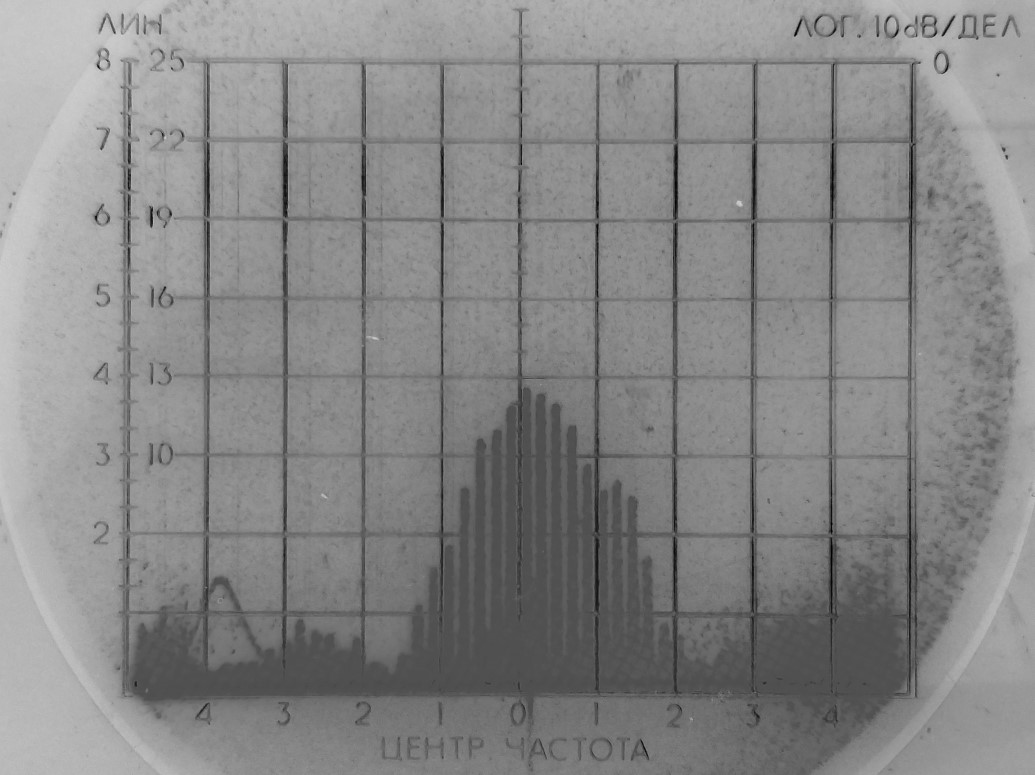
\includegraphics[scale=0.40]{Spectr_3}
	\caption{Фотография спектра с параметрами $\tau=100~\text{мкс}$, $m_x=5~\frac{\text{кГц}}{\text{дел}}$, $f_{повт}=1~\text{кГц}$} \label{Spectr_3}
	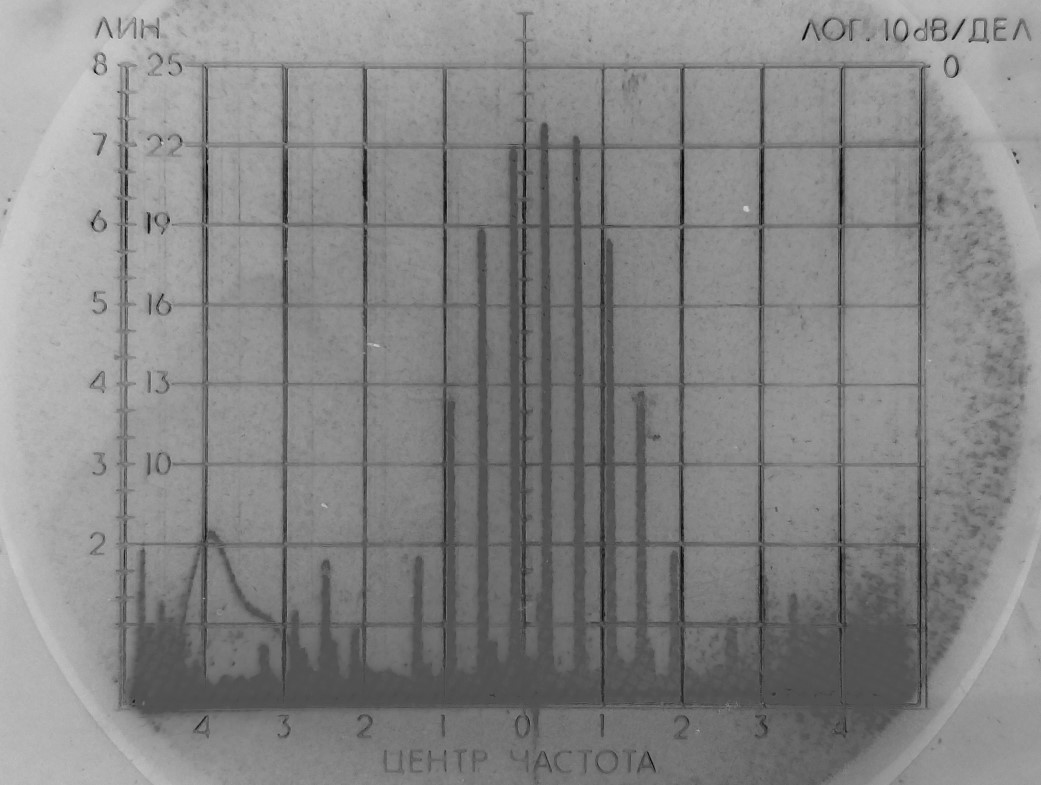
\includegraphics[scale=0.40]{Spectr_4}
	\caption{Фотография спектра с параметрами $\tau=100~\text{мкс}$, $m_x=5~\frac{\text{кГц}}{\text{дел}}$$f_{повт}=2~\text{кГц}$, } \label{Spectr_4}
\end{figure}

Сделаем промежуточный вывод о зависимости вида спектра цуга от параметров. Итак, (1) при одинаковых периодах $T$ и разных длительностях импульса $\tau$ спектры имеют одни и те же центр и плотность спектральных компонент, однако разную ширину; (2) при одинаковых $\tau$ и разных $T$ спектры имеют одни и те же центр и ширину, однако разную плотность спектральных компонент; (3) при одинаковых значениях $\tau$ и $T$ спектры цугов и прямоугольных импульсов имеют одни и те же ширину и плотность спектральных компонент, однако спектр прямоугольного импульса сииметричен относительно точки $\nu=0$, а спектр цуга -- относительно $\nu=\nu_0$ -- частоты несущей.

\subsection*{В. Исследование спектра гармонических сигналов, модулированных по амлитуде}

Соберём схему, показанную на рисунке \Ref{Device_3} и подготовим установку к проведению измерений. Изменяя глубину модуляции $m$, исследуем зависимость отношения амплитуды боковой линии спектра к амплитуде основной линии ($\frac{a_{\text{бок}}}{a_{\text{осн}}}$) от $m$ в диапазоне $m\in\left(0;1\right]$. Глубину модуляции $m$ будем расчитывать по формуле $m=\frac{2A_{max}-2A_{min}}{2A_{max}+2A_{min}},$ где $2A_{max}$ и $2A_{min}$ -- измеряемые на экране осциллографа удвоенные максимальная и минимальная амплитуды соответстенно. Полученные данные занесём в таблицу \Ref{Table_C}. Проведём оценку погрешностей. Для измерения амплитуды на экране осциллографа оценим погрешность в половину цены деления экранной сетки $\Delta A=0,13$, аналогично для сетки анализатора $\Delta a=0,17$. Для выражения для $m$ получим формулу $\sigma_m=\frac{2\Delta A\sqrt{\left(2A_{max}\right)^2+\left(2A_{min}\right)^2}}{\left(2A_{max}+2A_{min}\right)^2}$, а для отношения $\frac{a_{\text{бок}}}{a_{\text{осн}}}$ -- формулу $\sigma_{\frac{a_{\text{бок}}}{a_{\text{осн}}}}=\frac{\Delta a\sqrt{a_{\text{осн}}^2+a_{\text{бок}}^2}}{a_{\text{осн}}^2}$. Вычислим по ним погрешности и тоже внесём их в таблицу \Ref{Table_C}.

\begin{table}[h]
	\centering
	\caption{Зависимость относительной амплитуды боковой линии $\frac{a_{\text{бок}}}{a_{\text{осн}}}$ от глубины модуляции $m$} \label{Table_C}
	\begin{tabular}{|c|c|c|c|c|c|c|}
		\hline
		$2A_{min}$ & 2,8 & 2,2 & 1,6 & 1,2 & 0,8 & 0,0 \\ \hline
		$2A_{max}$ & 4,2 & 4,8 & 5,4 & 5,8 & 6,2 & 7,0 \\ \hline
		$m$ & 0,20 & 0,37 & 0,54 & 0,66 & 0,77 & 1,00 \\ \hline
		$\sigma_m$ & 0,03 & 0,03 & 0,03 & 0,03 & 0,03 & 0,04 \\ \hline
		$a_{\text{бок}}$ & 1,00 & 1,67 & 2,00 & 2,67 & 3,33 & 4,00 \\ \hline
		$a_{\text{осн}}$ & 7,67 & 7,67 & 7,67 & 7,67 & 7,67 & 7,67 \\ \hline
		$\frac{a_{\text{бок}}}{a_{\text{осн}}}$ & 0,13 & 0,22 & 0,26 & 0,35 & 0,43 & 0,52 \\ \hline
		$\sigma_{\frac{a_{\text{бок}}}{a_{\text{осн}}}}$ & 0,02 & 0,02 & 0,02 & 0,02 & 0,02 & 0,02 \\ \hline
	\end{tabular}
\end{table}

Приступим к обработке полученных данных. Построим график $\frac{a_{\text{бок}}}{a_{\text{осн}}}\left(m\right)$. Видим, что точки очень хорошо ложатся на прямую, поэтому найти наклон графика и его погрешность можно, используя МНК, и затем, используя этот результат, провести на графике прямую. Получим $k=0,497\pm0,013$. График приведён ниже на рисунке \Ref{Plot_C}. Исходя из этих результатов, можно убедиться, что $\frac{a_{\text{бок}}}{a_{\text{осн}}}=\frac{m}{2}$, т.е. совпадает с теоретическим предсказанием.

\begin{figure}[h]
	\centering
	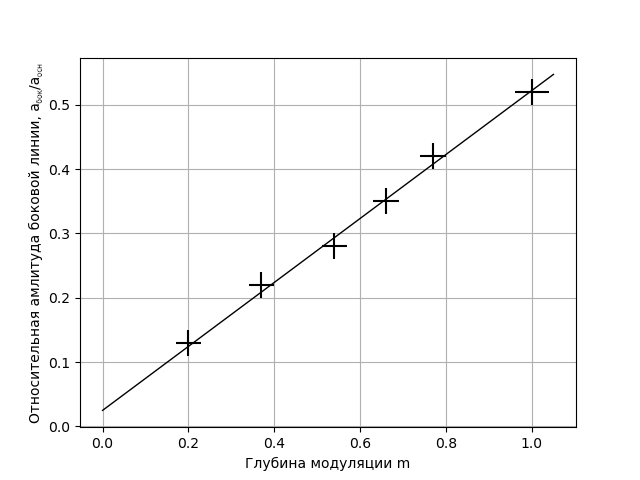
\includegraphics[scale=0.75]{Plot_C}
	\caption{График зависимости отношения амплитуды боковой линии спектра к амплитуде основной линии $\frac{a_{\text{бок}}}{a_{\text{осн}}}$ от глубины модуляции $m$. Прямая проведена с помощью МНК} \label{Plot_C}
\end{figure}

Наконец, посмотрим, как меняется спектр при $m\equiv1$ в зависимости от частоты модулирующео сигнала. Видим, что при увеличении частоты боковые линии становятся всё дальше от центральной.

\section*{Вывод}

В данной работе был изучен спектральный состав периодических электрических сигналов.

В первой части работы было проверено и экспериментально подтверждено соотношение неопределённостей $\tau\Delta\nu=1$ для прямоугольных импульсов. Были сделаны фотографии спектров с различными параметрами, качественно описаны зависимости регистрируемых картин от параметров.

Во второй части работы были исследованы спектры цугов гармонических колебаний, экспериментально подтвержджён тот факт, что при стремлении частоты повторения цугов к нулю спектр переходит в непрерывный, совпадающий с теоретическим предсказанием. Также сделаны фотографии спектров с различными параметрами, качественно описаны зависимости регистрируемых картин от параметров.

В последней части работы были исследованы спектры гармонических сигналов, модулированных по амплитуде. Экспериментально подтвержено соотношение $\frac{a_{\text{бок}}}{a_{\text{осн}}}=\frac{m}{2}$, качественно описаны зависимости регистрируемых картин от параметров.

Результаты оценки погрешностей говорят о хорошей точности использованных методов и корректном проведении эксперимента.

\end{document}
